\chapter{Hasil dan Pembahasan}

\par
Pengujian dilakukan dengan pakar dan pengguna biasa, sehingga skenario pengujian pun berbeda.
\section{Hasil Pengujian dengan Pakar Pariwisata}

\par
Dengan menggunakan skenario \ref{table:scenario}, berikut adalah hasil yang didapatkan dari pengujian dengan pakar:
\begin{center}
\small
\begin{longtable}{ |l|l|l|l|l|l| } 
\hline
\textbf{No} & \textbf{Lokasi pengguna} & \textbf{Waktu} & \textbf{Cuaca} & \textbf{No Uji} & \textbf{Presisi}\\
\hline
1	&	Alun-alun Cimahi	&	09:00	& bagus & 1 & 1\\
\hline
2	&	Alun-alun Cimahi	&	09:00	& kurang bagus & 1 & 1\\
\hline
3	&	Alun-alun Cimahi	&	09:00	& buruk & 1 & 1\\
\hline
4	&	Alun-alun Cimahi	&	13:00	& bagus & 2 & 1\\
\hline
5	&	Alun-alun Cimahi	&	13:00	& kurang bagus & 2 & 1\\
\hline
6	&	Alun-alun Cimahi	&	13:00	& buruk & 2 & 0.9\\
\hline
7	&	Alun-alun Cimahi	&	18:00	& bagus & 3 & 1\\
\hline
8	&	Alun-alun Cimahi	&	18:00	& kurang bagus & 3 & 1\\
\hline
9	&	Alun-alun Cimahi	&	18:00	& buruk & 3 & 0.7\\
\hline
10	&	Jalan Setiabudhi Bandung	&	09:00	& bagus & 1 & 1\\
\hline
11	&	Jalan Setiabudhi Bandung	&	09:00	& kurang bagus & 1 & 1 \\
\hline
12	&	Jalan Setiabudhi Bandung	&	09:00	& buruk & 1 & 0.9\\
\hline
13	&	Jalan Setiabudhi Bandung	&	13:00	& bagus & 2 & 1\\
\hline
14	&	Jalan Setiabudhi Bandung	&	13:00	& kurang bagus & 2 & 1\\
\hline
15	&	Jalan Setiabudhi Bandung	&	13:00	& buruk & 2 & 0.9\\
\hline
16	&	Jalan Setiabudhi Bandung	&	18:00	& bagus & 3 & 1\\
\hline
17	&	Jalan Setiabudhi Bandung	&	18:00	& kurang bagus & 3 & 0.9\\
\hline
18	&	Jalan Setiabudhi Bandung	&	18:00	& buruk & 3 & 0.7\\
\hline
19	&	Jalan Buah Batu	&	09:00	& bagus & 1 & 1\\
\hline
20	&	Jalan Buah Batu	&	09:00	& kurang bagus & 1 & 1\\
\hline
21	&	Jalan Buah Batu	&	09:00	& buruk & 1 & 0.9\\
\hline
22	&	Jalan Buah Batu	&	13:00	& bagus & 2 & 1\\
\hline
23	&	Jalan Buah Batu	&	13:00	& kurang bagus & 2 & 1\\
\hline
24	&	Jalan Buah Batu	&	13:00	& buruk & 2 & 0.8\\
\hline
25	&	Jalan Buah Batu	&	18:00	& bagus & 3 & 1\\
\hline
26	&	Jalan Buah Batu	&	18:00	& kurang bagus & 3 & 0.8\\
\hline
27	&	Jalan Buah Batu	&	18:00	& buruk & 3 & 0.6\\
\hline
\caption{Tabel skenario pengujian dengan pakar}
\label{table:result-1}
\end{longtable}
\end{center}

\begin{figure}[h!]
    \centering
    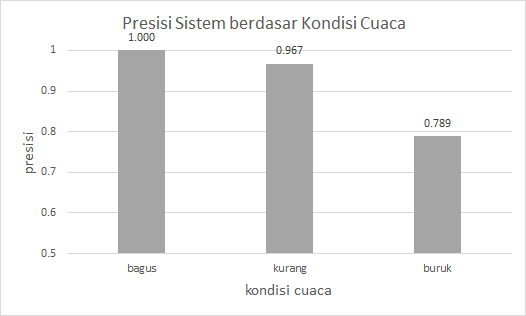
\includegraphics[scale=0.7]{img/precision_weather.png}
    \caption{Mean presisi sistem berdasar kondisi cuaca}
    \label{fig:p_weather}
\end{figure}


\begin{figure}[h!]
    \centering
    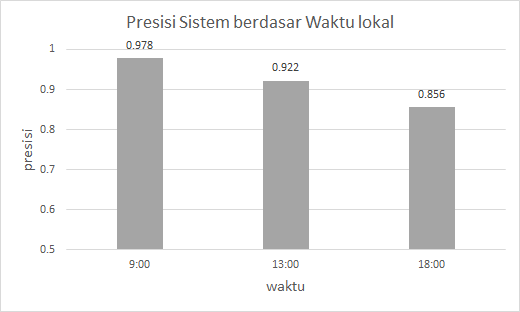
\includegraphics[scale=0.7]{img/precision_time.png}
    \caption{Mean presisi sistem berdasar waktu lokal pengujian}
    \label{fig:p_time}
\end{figure}

\section{Hasil Pengujian dengan Pengguna Biasa}
\begin{figure}[h!]
    \centering
    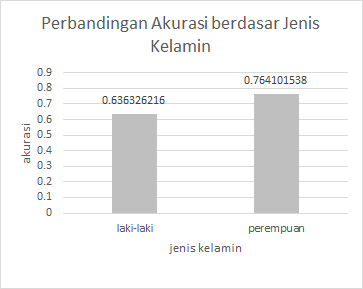
\includegraphics[scale=1]{img/accuracy-gender.png}
    \caption{Akurasi sistem berdasar jenis kelamin}
    \label{fig:accuracy-gender}
\end{figure}

\begin{figure}[h!]
    \centering
    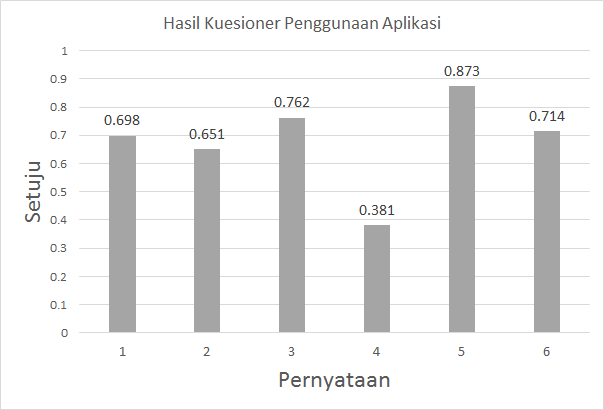
\includegraphics[scale=0.7]{img/hasil_kuesioner.png}
    \caption{Hasil kuesioner pengguna aplikasi}
    \label{fig:quest}
\end{figure}